\chapter{MRCVC e ICESym}

El Simulador de Motores de Combustión Interna (ICESym) permite la simulacion de
motores tanto alternativos como rotativos en general y el MRCVC en particular.
%
En su código se incluyen modelos de la geometría del motor, la transferencia
de calor y el solape de cámaras.

En este capítulo se describe brevemente el ciclo operativo de MRCVC, los
aspectos generales de ICESym que hacen a la simulación del mismo, cómo se
utilizó el simulador y las modificaciones que se realizaron para este trabajo.

\section{Simulación computacional del ciclo termodinámico del MRCVC}

El MRCVC es un motor rotativo de combustión interna encendido por chispa, en el
que gran parte de la misma ocurre a volumen constante.
%
ICESym utiliza modelos unidimensionales para simular el flujo en los conductos
de admisión/escape y modelos cero dimensionales o termodinámicos para la cámara
de combustión, la transferencia de calor y el modelado de la fricción.
%
Además, incluye un modelo para el solape entre cámaras~\cite{lopez16} entre
otras modificaciones particulares al MRCVC.\@

Con el objetivo de poder simular con más detalle el ciclo del motor, se ha
modificado el código de ICESym para permitir el uso de modelos de coeficiente
de descarga dependientes de dos variables: presión y alzada de válvula, de modo
que $Cd = f(L_v, \Delta P)$.
%
En trabajos anteriores se tienen estudios más detallados del MRCVC, por lo que
aquí se presenta de manera breve los aspectos geométricos y mecánicos del motor
que son relevantes a este trabajo.

\subsection{Geometría}
%
La geometría del MRCVC permite que gran parte de la combustión se de a volumen
constante\cite{mrcvc_geom}, como se puede ver en la figura~\ref{fig:vol_constante},
en donde se esquematiza la variación del volumen con respecto al ciclo.

\begin{figure}
    \centering
    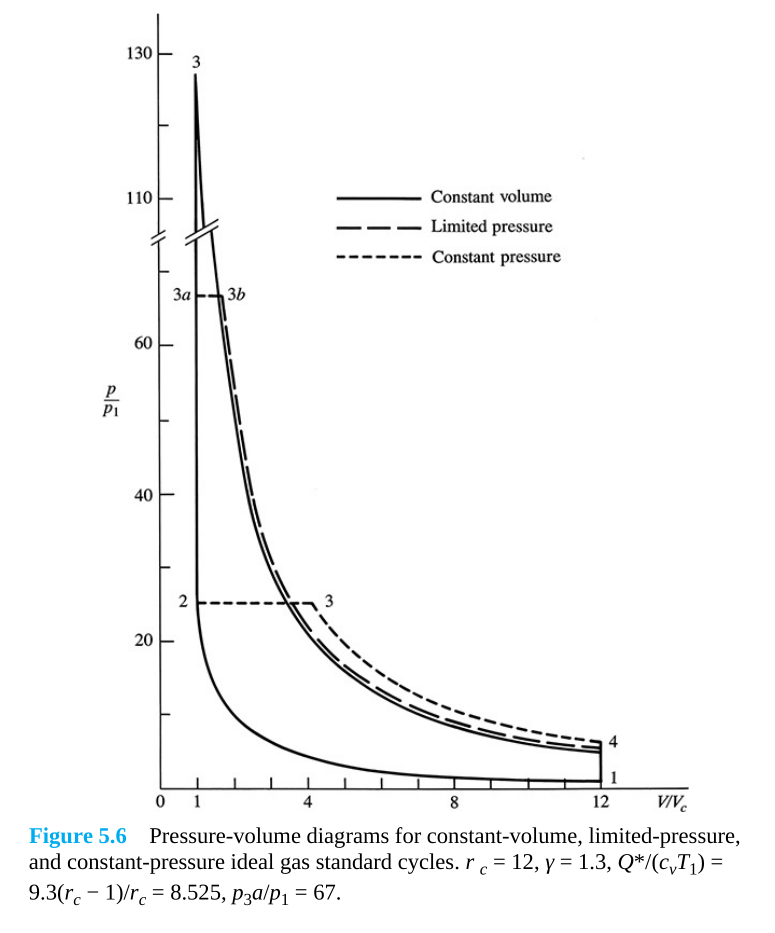
\includegraphics[width=0.7\textwidth]{comparacion_ciclos.png}
    \caption{Comparación de ciclos ideales (cambiar por una imagen propia)}\label{fig:comparacion_ciclos}
\end{figure}


Para un motor de $n$ paletas de radio de punta nulo, la geometría como función
del ángulo del cigüeñal queda totalmente definida por el radio de trayectoria de
paletas $R$, semiancho de paletas $r$ y altura de cámara $h$.

\begin{figure}
    \centering
    \begin{tikzpicture}
        \begin{axis}[
            xlabel=Angulo $(deg)$,
            ylabel=Volumen $(mm^3)$,
            grid=major,
            mark size=0pt,
        ]
        \addplot table [x=Angle,y=Volume] {data/vol.dat};
        \end{axis}
    \end{tikzpicture}
    \caption{Combustión a volumen constante}\label{fig:vol_constante}
\end{figure}

La geometría utilizada para este trabajo se resumen en la
tabla~\ref{tab:geom_mrcvc} y se ilustra en la figura~\ref{fig:geom_mrcvc}.
%
Esta geometría es la continuación de la utilziada en trabajos anteriores, con la
cual se realizó parte del prediseño del sistema de intercambio de gases.

\begin{table}
    \centering
    \begin{tabular}{rcc} \toprule
        Parámetro & Valor                            & Unidades \\ \midrule
        n         & \lua{tex.print(myData.n)}        & unidades \\
        R         & \lua{tex.print(myData.R)}        & mm \\
        r         & \lua{tex.print(myData.r)}        & mm \\
        $h_c$     & \lua{tex.print(myData.hc)}       & mm \\
        rc        & \lua{tex.print(myData.rc)}       & --- \\
        V0        & \lua{tex.print(myData.V0)}       & $cm^3$ \\
        $R_i$     & \lua{tex.print(trunc(myData.Ri))} & mm \\
        $R_e$     & \lua{tex.print(trunc(myData.Re))} & mm \\
    \end{tabular}
    \caption{Geometría del MRCVC}\label{tab:geom_mrcvc}
\end{table}

Los ángulos que determinan el reglaje de los puertos de admisión y escpe son los
de inicio y de cierre del puerto.
%
Como ejemplo, la posición del puerto de escape queda determiada por los  valores
EIA y EFA como se ve en la figura~\ref{fig:angulos_escape}.

\begin{figure}
    \centering
    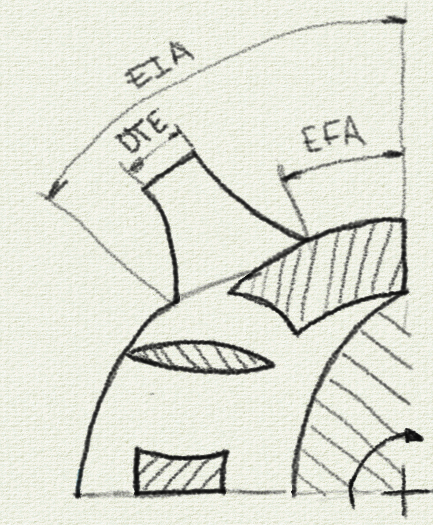
\includegraphics[width=0.5\textwidth]{angulos_escape.png}
    \caption{Puerto de escape}\label{fig:angulos_escape}
\end{figure}

Como se puede ver en la figura~\ref{fig:primeros_puertos}, se buscó suavizar los
vértices en donde la pared del puerto intersecta la cámara de combustión.

\subsection{Ciclo operativo}
%
La variación de la geometría y el funcionamiento en detalle de ICESym, así como
también el modelo de solape de cámaras desarrollado para el uso con el MRCVC.\@
%
Para una misma relación de compresión, una combustión a volumen constante
alcanza valores de presión y temperatura mayores en comparación a otros ciclos.
%
En la figura~\ref{fig:comparacion_rendimientos} se ve como para una $r_c$ dada,
el ciclo a volumen constante tiene el mayor rendimiento.

\begin{figure}
    \centering
    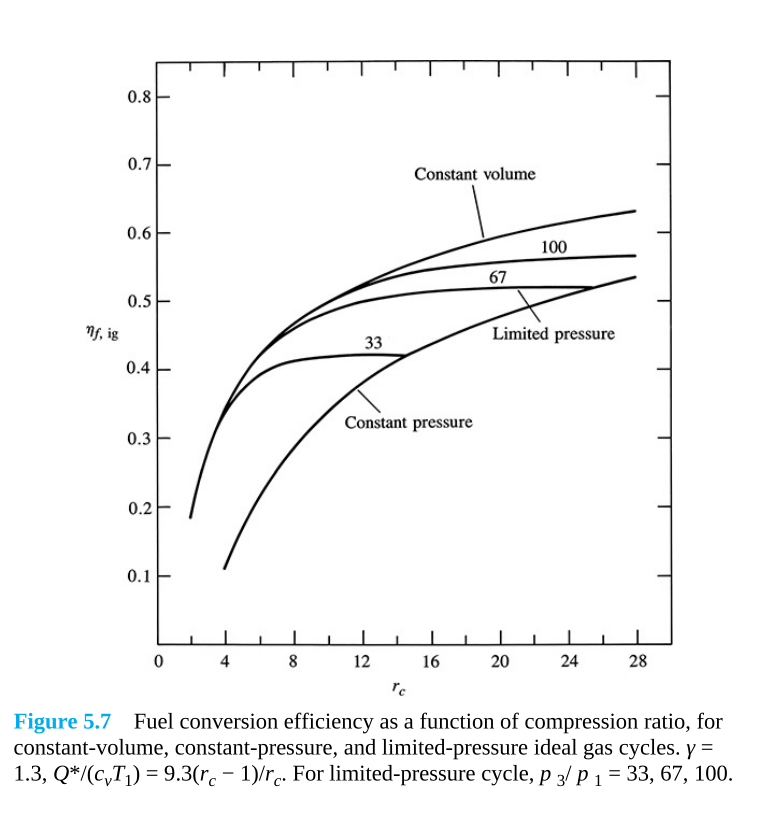
\includegraphics[width=1\textwidth]{rendimiento_conv_comb.png}
    \caption{Comparación de rendimientos (cambiar por una imagen propia)}\label{fig:comparacion_rendimientos}
\end{figure}

El indicador que se tomará como referencia para evaluar y comparar diferentes
geometrías es el rendimiento volumétrico ($\eta_v$), este parámetro se define
como:

\begin{equation}
    \eta_v = \frac{m_a}{\rho_{a,i}V_d}
\end{equation}

Dónde:
%
\begin{description}
    %
    \item[$m_i$] es la masa de mezcla fresca inductada
        %
    \item[$\rho_{a,i}$] es la densidad del aire en el puerto de admisión
        %
    \item[$V_d$] es el volumen desplazado
        %
\end{description}

El rendimiento volumétrico tiene una dependencia compleja de varios factores,
este parámetro es el que da forma a las curvas de \emph{performance} que se
suelen ver en literatura ya que indica la cantidad de mezcla fresca disponible
para la combustión. 
%
% En caso de motores de inyección directa (tanto de CI SI)
% NOTA: no se que quise poner aca, voy a tener que leerlo con mas de talle de
% nuevo

La combustión es estequeométrica con $a_{weibe}=5$ y $m_{weibe}=2$, el combustible utilizado
es \emph{isooctano} con las siguientes características:
\begin{itemize}
    \item $y = 2.25$
    \item $H_{vap} = 2.25 MJ/kg$
    \item $Q_{fuel} = 44 MJ/kg_f$
\end{itemize}

La temperatura de pared se asume en 450K.


\section{Sistemas de intercambio de gases}
%
\subsection{Área de referencia}
%
El área de referencia utilizada por ICESym es el área de cortina.

\begin{equation}
  \label{eq:Ar}
  A_R = A_C = \pi D_v L_v
\end{equation}

\begin{figure}
  \centering
  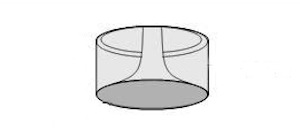
\includegraphics[width=0.5\textwidth]{valve_curtain.jpg}
  \caption{Área de cortina}\label{fig:area_cortina}
\end{figure}

Dónde $D_v$ es el diámetro de la válvula y $L_v$ es la alzada de la misma.

El área de referencia utilizada en este trabajo es el área del puerto expuesta a
la cámara, que se calcula como el producto entre la longitud o cuerda del puerto
descubierta en el plano del estator $l_v$ y la altura de la ranura del puerto
$h_p=29.4mm$.
%
Con esto el área de válvula utilizada en ICESym es:
\begin{equation}
  \label{eq:fv}
  F_v = Cd_{int}*0.0294*L_v
\end{equation}

En dónde $Cd_{int}$ es el coeficiente de descarga interpolado del mapa, para un apertura
y diferencial de presión dado.

% NOTA: aca hay que meter un croquis

% \subsection{Solape de cámaras}
%
Tanto al inicio como al cierre del puerto ocurre solape de cámaras, por lo que
en estos intervalos angulares hay un valor de $C_D$ para cada cámara.
%
Este se calcula con el flujo másico que atraviesa los parches correspondientes
a cada cámara y el área de puerto expuesta por cada cámara.
% NOTA:A ver nota 8

\section{CAD}
%
El modelo 3D de los puertos de admisión, escape y los componentes internos del
motor que afectan el flujo y son relevantes a la flujometría se realizaron con
FreeCAD\cite{freecad} para generar un archivo en formato \emph{.BREP} para cada
posición analizada.
%
Estos archivos son importados al software salome\cite{salome}, ese permite
generar una malla cerrada que se puede utilizar para OpenFOAM.\@
%
Antes de generar la malla se apliacn los nombres de los parches, en los que
luego se toman de referencia para aplicar las reglas para realizar el
refinamiento con snappyHexMesh, aplicar condiciones de contorno, iniciales y
demás.
%
Se genera la malla con el mallador NETGEN 1D-2D-3D y se exporta parche por
parche en formato \emph{ASCII.stl}.

%
El archivo \emph{stl} se utiliza en OpenFOAM para generar la malla con
\emph{snappyHexMesh}.

Dada la cantidad de geometrías posibles y el tiempo que toma el proceso, se
realizaron algunas simplificaciones, las cuales se listan a continuación.

% \subsection{Geometría}
%
\begin{enumerate}

    \item La interfaz entre los puertos de admisón y escape con sus respectivos
        conductos de conexión con la atmósfera es de sección circular.
        %
    \item La altura de la ranura se adopta en 2/3 del alto de la cámara, siendo
        $h_c=\lua{tex.print(myData.hc)}\ mm$.
        %
    \item El eje del puerto se hace perpendicular a una línea que pasa entre el
        centro del motor y el la línea media del puerto.
        %

\end{enumerate}

% En este capítulo describo como es el procedimiento realizado en cada paso de
% la optimización:

% -> optimización algoritmo genético y simulación con icesym, tendría que
%    explicar como funciona icesym y el optimizador
% -> freecad + salome
% -> openfoam
\section{Metodología}
%
Se simulará un MRCVC de 3 paletas usando el simulador de motores de combustión
interna ICESym~\cite{icesym} con el propósito de obtener curvas de rendimiento
volumétrico.
%
Estas serán el principal criterio para evaluar el diseño de los sistemas de
intercambio de gases, que consisten de los puertos y conductos.
%
La geometría se optimizará mediante un algoritmo genético, el cual transforma
los datos de rendimiento volumétrico en un puntaje representativo de cada
motor.


La simulación con ICESym requiere del conocimiento previo de los coeficientes
de descarga de los puertos, en la primer iteracion se asume un valor constante
para cada puerto, siendo 0.7 y 0.75 para admisión y escape respectivamente.
%
Se utilizará la geometría obtenida en esta primer iteración para crear modelos
en CAD de los puertos de admisión y escape, junto con una porción de la cámara
pde combustion para realizar flujometrías virtuales.
%
De este modo se puede obtener los coeficientes de descarga de cada puerto en
distintos grados de apertura.

Con el resutlado de las flujometrias se contruye un mapa del $C_D$ en función
de la alzada, que representa la posición del puerto y la diferencia de presión
entre el puerto y la cámara de combustión.

Este mapa se introduce en ICESym y se vuelve a realizar el proceso de optimización
con el algoritmo genético.

\section{Modificaciones a ICESym}
%
Para poder realizar lo indicado en el apartado anterior, fue necesario
realiziar algunas modificaciones menores al simulador de motores, tales como:
modificar los arhcivos de salida para facilitar la lectura y procesamiento de
datos, incluir una opción para elegir entre un modelo de Cd de una o dos
variables, modificar el área de referencia y  agregar una interpolación
bilineal de los datos de Cd.

\subsection{Flujo a través de los puertos}
%
Para tener un mejor modelado del flujo de gas a través dee los puertos de los
puertos de admisión y escape, se introdujo una opción para poder ejecutar
ICESym con un modelo del coeficiente de descarga que dependa de dos variables,
diferencia de presión y \emph{alzada} o apertura del puerto $C_D = f(\Delta P;
lv)$.
%
Esto significó agregar una opcion que permita seleccionar entre un Cd que
depende únicamente de una o dos variables.

Con esto se construye una mapa del coeficiente de descarga de la forma $C_d =
f(lv, dp)$, que se utiliza en \emph{def\_valve.f90} para calcular el área
efectiva de la válvula.

La interpolación bilineal se realiza sobre una malla rectangular, con esto se
realiza simplemente una interpolación lineal entre dos valores en planos con
datos conocidos.

% \begin{lstlisting}[language=fortran]
%    SUBROUTINE interpolant2d(x, y, z, xi, yi, zi)
%       [...]
%       nx = SIZE(x)
%       IF (xi .LE. x(1)) THEN ! <=
%          CALL interpolant(y, z(1, :), yi, zi)
%          RETURN
%       ELSE IF (xi .GE. x(nx)) THEN  ! >=
%          CALL interpolant(y, z(nx, :), yi, zi)
%          RETURN
%       END IF
%       i = iminloc(dabs(x - xi))
%       IF (x(i) .GT. xi) i = i - 1 ! >
%       CALL interpolant(y, z(i, :), yi, z_aux(1))   ! z1=f(x1,yi)
%       CALL interpolant(y, z(i + 1, :), yi, z_aux(2)) ! z2=f(x2,yi)
%       CALL interpolant(x(i:i + 1), z_aux, xi, zi)   ! zi=f(xi,yi)
%       [...]
%    END SUBROUTINE interpolant2d
% \end{lstlisting}
\begin{algorithm}
 \caption{Interpolación bi-lineal}\label{algo:bilineal}
    \SetAlgoLined
    \SetKwFunction{Size}{Size}
    \SetKwFunction{Interpolant}{Interpolant}

    \KwIn{\\
        $\vec{x}, \vec{y}$: valores de $x, y$ en los que se conoce el valor en $z$.\\
        $\vec{z}$: valores conocidos de $z$.\\
        $x_i, y_i$: puntos donde se quiere interpolar.\\
      }
    \KwResult{Devuelve el valor interpolado de $z_i$.}
    $n_x \Leftarrow Size(x)$\;
    \eIf{
      $x_i \geq x_{n_x}$
    }{
      $z_i \Leftarrow Interpolant(y, z[1,:], y_i)$\;
      \Return\;
    }{
      $z_i \Leftarrow Interpolant(y, z[n_x,:], y_i)$\;
      \Return\;
    }
    $i \Leftarrow iminloc(dabas(x-x_i))$\;

\end{algorithm}

Si bien hay otros métodos para estimar el valor de Cd para dos valores $(\Delta
P; l_v)$, este método es sencillo y da resultados satisfactorios.
%
En la figura~\ref{fig:bilineal} se muesta un ejemplo del error obtenido
con este método para interpolar una función de prueba 
$\sin(\sqrt(x^2 + y^2))$.

\begin{figure}
    \centering
    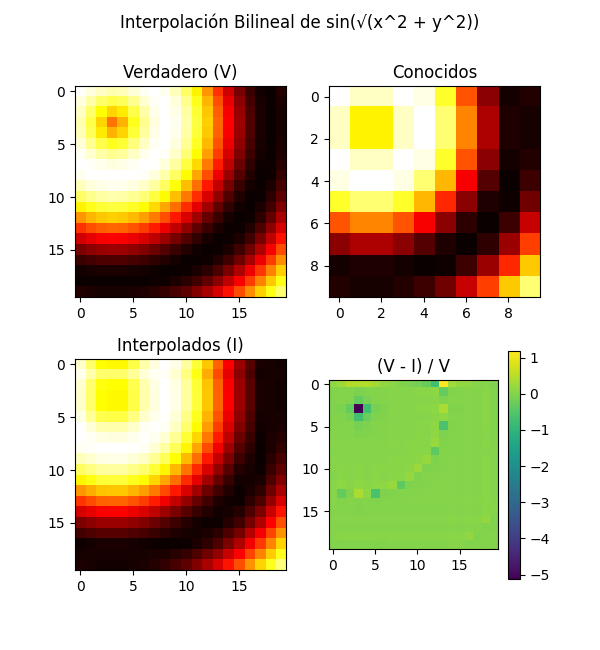
\includegraphics[width=0.7\textwidth]{bilineal.png}
    \caption{Interpolación bilineal de $\sin(\sqrt(x^2 + y^2))$}\label{fig:bilineal}
\end{figure}

La malla rectangular se realizará a partir de los valores de $C_d$ que se
obtengan de flujometrías con \emph{OpenFoam}~\cite{openfoam}.
%
Debido al costo computacional que requieren la flujoemtría, solo una cantidad
reducida de puntos se obtendrá con este método, las combinaciones de $(\Delta
P; l_v)$ ensayadas se indican con detalle en apartados posteriores.
%
Esto significa que se tiene como punto de partida una malla no rectangular, por
lo que se utiliza un método intermedio para obtener una matriz de puntos que
pueda ser leido por la interpolación bilineal.

Se probaron dos métodos para realizar la interpolación, el método del punto
más cercano y la interpolación por la suma de la inversa de la distancia o 
IDW por sus siglas en inglés (\emph{Inverse Distance Weighting}).
%
Estos métodos se combinan con suavizados con un promedio móvil de los $n$
valores más cercanos.

El método del punto más cercano consiste en asignar para cada par $(x, y)$
el valor conocido más cercano, el algoritmo es como se indica a continuación:

\begin{algorithm}
 \caption{Interpolación por punto más cercano}\label{algo:mas_cercano}
    \SetAlgoLined

    \KwIn{\\
        $V_x, V_y$: valores de $x, y$ en los que se conoce el valor en $z$.\\
        $V_z$: valores conocidos de $z$.\\
        $I_x$: $n$ puntos de $x$ donde se quiere interpolar\\
        $I_Y$: $m$ puntos de $y$ donde se quiere interpolar\\
        }

    \KwResult{Devuelve una matriz $I_{[n,m]}$ con los valores interpolados,
      donde cada punto $I(x,y)$ se le asigna al valor de $V_Z$ más cercano
      conocido. Da como resultado superficies escalonadas.}

    \BlankLine
     $I=zeros_{[n,m]}$\;
     \For{$i \gets 0$\KwTo$n$}{
        \For{$j \gets 0$\KwTo$m$}{
          $d = \sqrt{{(V_x - I_{xi})}^2 + {(V_y - I_{yj})}^2}$\;
            $I[i,j] = v_z[\min(d)]$\;
        }
     }
\end{algorithm}

La interpolación IDW consiste en asignar a cada punto el resultado de un promedio
de los valores cercanos al punto en cuestión, ponderado por la distancia al valor
elevado a un exponente arbitrario $p$.
%
Cuanto mayor sea el valor de $p$, más sensible es el método a los valores cercanos,
la formulación de este método se ve en la ecuación~\ref{eq:idw}.

\begin{equation}
    f_p = \frac{\sum_{i=1}^{n} \frac{z_i}{d_i^p}} {\sum_{i=1}^{n} \frac{1}{d_i^p}}
    \label{eq:idw}
\end{equation}

La función utilizada para calcular esto es esto es:

\begin{algorithm}
    \caption{Interpolación IDW}\label{algo:IDW}
    \SetAlgoLined

    \KwIn{\\
        $V_x, V_y$: valores de $x, y$ en los que se conoce el valor en $z$.\\
        $V_z$: valores conocidos de $z$.\\
        $I_x$: $n$ puntos de $x$ donde se quiere interpolar\\
        $I_Y$: $m$ puntos de $y$ donde se quiere interpolar\\
        $p$: potencia a la que se eleva cada peso\\
        }

    \KwResult{Interpolación ponderada por inverso de la distancia. Dependiendo
      del valor de p, se obtienen valores más o menos suavizados.}

    \BlankLine
    $I=zeros_{[n,m]}$\;
    \For{$i \gets 0$\KwTo$n$}{
        \For{$j$\gets 0 \KwTo$m$}{
          $d = {\left[{(V_x - I_{xi})}^2 +{(V_y - I_{yj})}^2\right]}^{\frac{p}{2}}$\;
          \eIf{$\exists i : d[i] = 0$}{
            $I[i, j] = V_z[i]$\;
          }{
            $I[i,j] = \frac{\sum{V_{zi}/d_i}}{\sum \frac{1}{d}}$\;
          }
        }
     }
\end{algorithm}


\begin{figure}
    \centering
    \begin{subfigure}{0.4\textwidth}
        \centering
        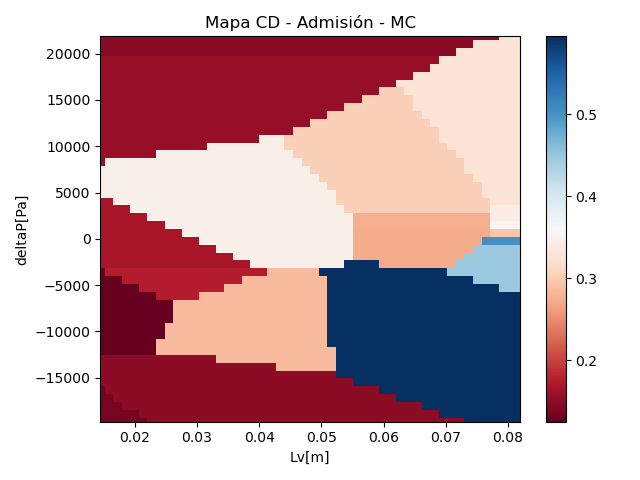
\includegraphics[width=\textwidth]{mapa_cd/mc_mapa_adm.png}
        \caption{Punto Más Cercano sin suavizar}
    \end{subfigure}
    \hfill
    \begin{subfigure}{0.4\textwidth}
        \centering
        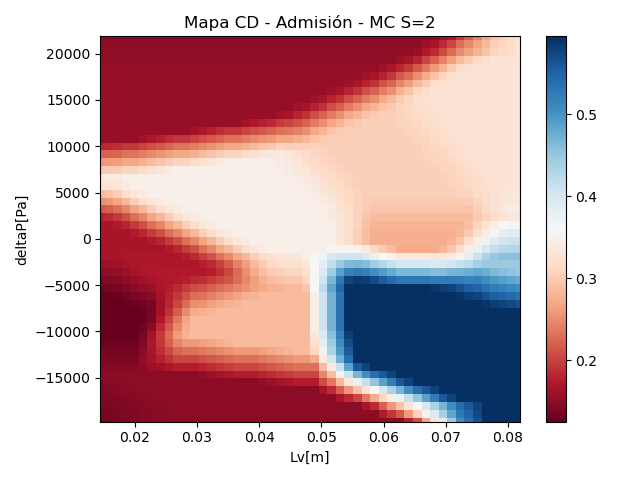
\includegraphics[width=\textwidth]{mapa_cd/mc_s2_mapa_adm.png}
        \caption{Más Cercano ($S=2$)}
    \end{subfigure}
    \hfill
    \begin{subfigure}{0.4\textwidth}
        \centering
        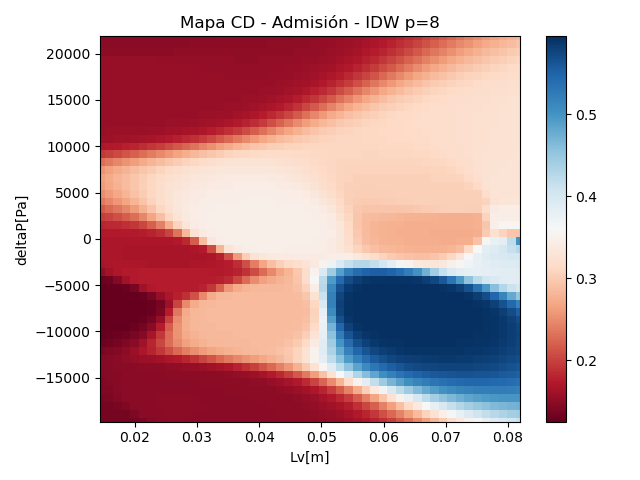
\includegraphics[width=\textwidth]{mapa_cd/idw8_mapa_adm.png}
        \caption{IDW ($p=8$)}
    \end{subfigure}
    \hfill
    \begin{subfigure}{0.4\textwidth}
        \centering
        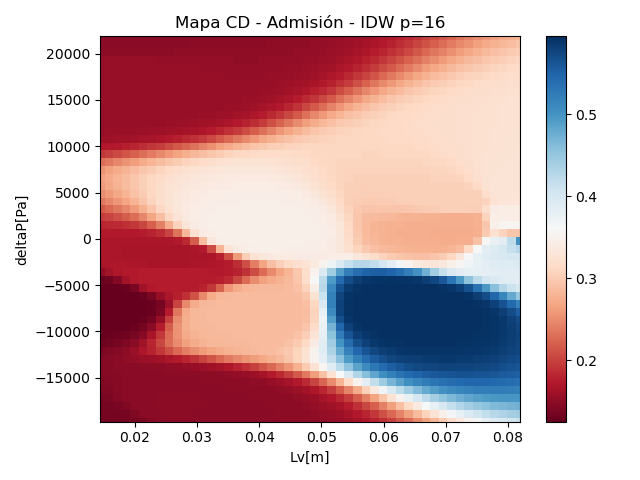
\includegraphics[width=\textwidth]{mapa_cd/idw16_mapa_adm.png}
        \caption{IDW ($p=16$)}
    \end{subfigure}
    \caption{Comparación de interpolaciones}\label{fig:mapas_interpolados}
\end{figure}
